\chapter{Proof by Picture}

\begin{quote}
A picture is worth a thousand words.

\hfill---Unknown
\end{quote}


\section{Basic Set Theory}

The word \textit{set} has more definitions in the dictionary than any
other word. In our case we'll use the following definition:

\begin{dfn}\index{set} 
A \textbf{set} is any collection of elements for which we can always
tell whether an element is in the set or not.
\end{dfn}

\begin{ques} 
What are some examples of sets? What are some examples of things that
are not sets?
\end{ques}
\QM

If we have a set $X$ and the element $x$ is inside of $X$, we write:
\[
x\in X\index{e@$\in$}\index{set theory symbols!in@$\in$}
\]
This notation is said ``$x$ in $X$.'' Pictorially we can imagine this
as:
\[
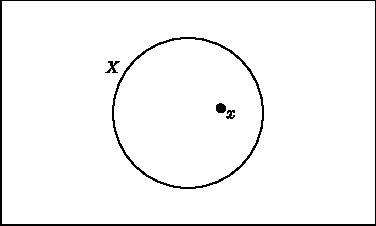
\includegraphics{../graphics/set1.pdf}
\]

\begin{dfn} 
A \textbf{subset}\index{subset} $Y$ of a set $X$ is a set $Y$ such
that every element of $Y$ is also an element of $X$. We denote this
by:
\[
Y\subset X\index{set theory symbols!subset@$\subset$}
\] 
\end{dfn}

If $Y$ is contained in $X$, we will sometimes loosely say that $X$ is
\textit{bigger} than $Y$.

\begin{ques} 
Can you think of a set $X$ and a subset $Y$ where saying $X$ is bigger
than $Y$ is a bit misleading?
\end{ques}
\QM

\begin{ques} 
How is the meaning of the symbol $\in$ different from the meaning of
the symbol $\subset$?
\end{ques}
\QM


\subsection{Union}


\begin{dfn}\index{union}\index{u@$\cup$}\index{set theory symbols!union@$\cup$} Given two sets $X$ and $Y$, $X$ \textbf{union} $Y$ is the set of all the elements in $X$ or $Y$. We denote this by $X\cup Y$.
\end{dfn}

Pictorially, we can imagine this as:

\[
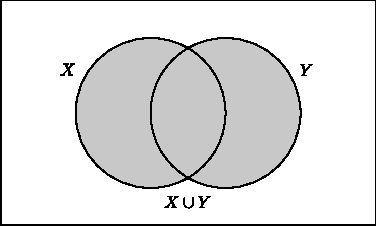
\includegraphics{../graphics/set2.pdf}
\]



\subsection{Intersection}

\begin{dfn}\index{intersection}\index{set theory symbols!intersection@$\cap$} Given two sets $X$ and $Y$, 
$X$ \textbf{intersect} $Y$ is the set of all the elements that are simultaneously in $X$ and in $Y$. We denote this by $X\cap Y$. 
\end{dfn}

Pictorially, we can imagine this as:
\[
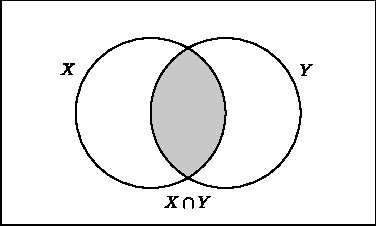
\includegraphics{../graphics/set3.pdf}
\]

\begin{ques} Consider the sets $X$ and $Y$ below:
\[
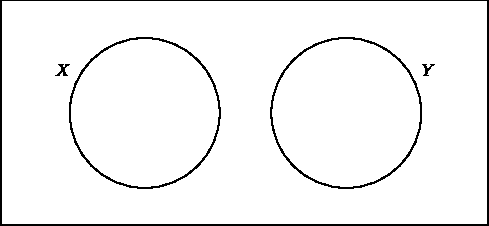
\includegraphics{../graphics/set4.pdf}
\]
What is $X\cap Y$?
\end{ques}

I'll take this one: Nothing! We have a special notation for the set with no elements, it is called the \index{empty set}\textbf{empty set}. We denote the empty set by the symbol $\emptyset$.\index{set theory symbols!emptyset@$\emptyset$}




\subsection{Complement}

\begin{dfn}\index{complement}\index{set theory symbols!complement@$-$} Given two sets $X$ and $Y$, 
$X$ \textbf{complement} $Y$ is the set of all the elements that are in $X$ and are not in $Y$. We denote this by $X-Y$.
\end{dfn}

Pictorially, we can imagine this as:
\[
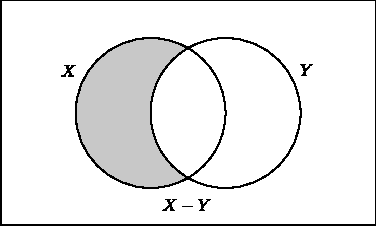
\includegraphics{../graphics/set5.pdf}
\]

\begin{ques} Check out the two sets below:
\[
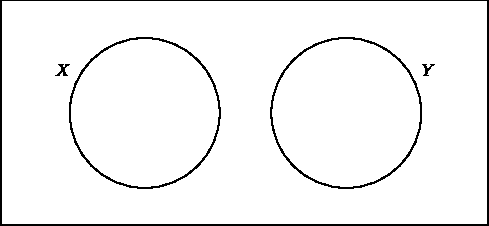
\includegraphics{../graphics/set4.pdf}
\]
What is $X-Y$? What is $Y-X$?
\end{ques}
\QM


\subsection{Putting Things Together}

OK, let's try something more complex:

\begin{ques} Prove that:
\[
X\cup (Y \cap Z) = (X \cup Y)\cap (X \cup Z)
\]
\end{ques}

\begin{proof} 
Look at the left-hand side of the equation first. We can represent the
elements in $Y\cap Z$ with shaded region in the following diagram:
\[
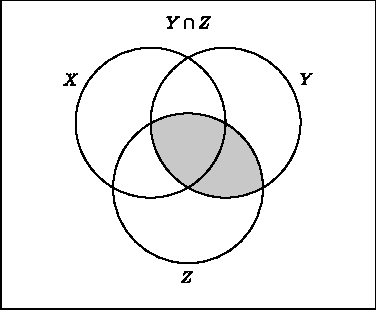
\includegraphics{../graphics/setproof.pdf}
\]
So the union of this region with $X$ is represented the shaded
region in this diagram.
\[
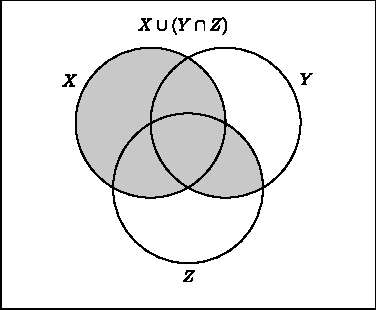
\includegraphics{../graphics/setproof1.pdf}
\]
Now, looking at the right-hand side of the equation, $X\cup Y$ is
represented by this shaded region:
\[
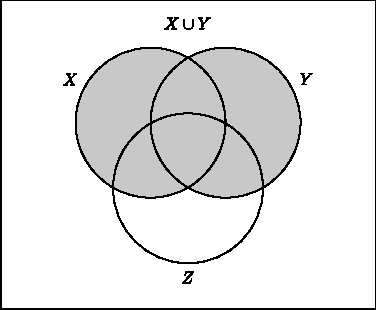
\includegraphics{../graphics/setproof2.pdf}
\]
And $X\cup Z$ is represented by this shaded region:
\[
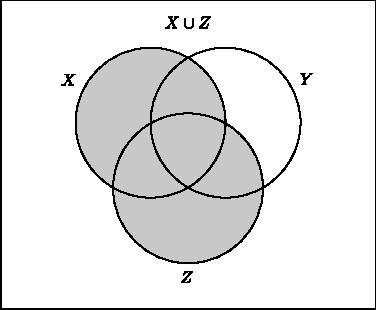
\includegraphics{../graphics/setproof3.pdf}
\]
The region shaded in both of the diagrams, which is the
intersection of $X\cup Y$ and $X\cup Z$, is represented by the shaded
region below.
\[
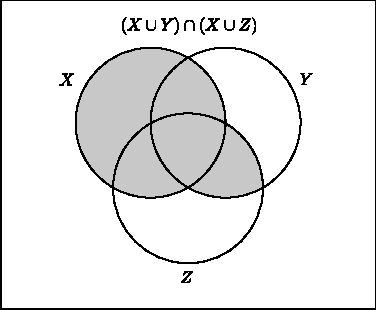
\includegraphics{../graphics/setproof4.pdf}
\]
Comparing the diagrams representing the left-hand and right-hand sides
of the equation, we see that the same regions are shaded, and so we
are done.
\end{proof}

\newpage

\subsection*{Problems for Section~\thesection}\hrule\vspace{1ex}
\begin{enumerate}
\item Given two sets $X$ and $Y$, explain what is meant by $X\cup Y$.
\item Given two sets $X$ and $Y$, explain what is meant by $X\cap Y$.
\item Given two sets $X$ and $Y$, explain what is meant by $X - Y$.
\item Explain the difference between the symbols $\in$ and $\subset$.
\item If we let $X$ be the set of ``right triangles'' and we let $Y$ be the set of ``equilateral triangles'' does the picture below show the relationship between these two sets?
\[
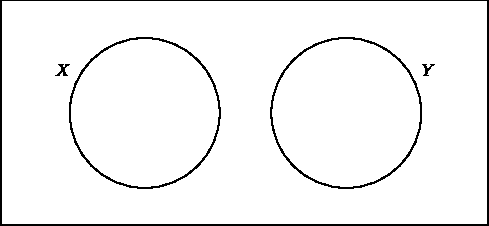
\includegraphics{../graphics/set4.pdf}
\]
Explain your reasoning.
\item If $X = \{1,2,3,4,5\}$ and $Y = \{3,4,5,6\}$ find:
\begin{enumerate}
\item $X\cup Y$
\item $X\cap Y$
\item $X-Y$
\item $Y-X$
\end{enumerate}
In each case explain your reasoning. 
\item Let $n\Z$ represent the integer multiples of $n$. So for example:
\[
3\Z = \{\dots,-12,-9,-6,-3,0,3,6,9,12,\dots\}
\]
Compute the following:
\begin{enumerate}
\item $3\Z\cap 4\Z$
\item $2\Z\cap 5\Z$
\item $3\Z\cap 6\Z$
\item $4\Z\cap 6\Z$
\item $4\Z\cap 10\Z$
\end{enumerate}
In each case explain your reasoning. 
\item Make a general rule for intersecting sets of the form $n\Z$ and
  $m\Z$. Explain why your rule works.
\item Prove that:
\[
X = (X\cap Y) \cup (X-Y)
\]
\item Prove that:
\[
X-(X-Y) = (X\cap Y)
\]
\item Prove that:
\[
X \cup (Y-X) = (X\cup Y)
\]
\item Prove that:
\[
X \cap (Y-X) = \emptyset
\]
\item Prove that:
\[
(X-Y)\cup (Y-X) = (X\cup Y)-(X\cap Y)
\]
\item Prove that:
\[
X\cup (Y \cap Z) = (X \cup Y)\cap (X \cup Z)
\]
\item Prove that:
\[
X\cap (Y \cup Z) = (X \cap Y)\cup (X \cap Z)
\]
\item Prove that:
\[
X - (Y \cap Z) = (X -Y)\cup (X - Z)
\]
\item Prove that:
\[
X - (Y \cup Z) = (X -Y)\cap (X -Z)
\]
\item If $X\cup Y = X$, what can we say about the relationship between the sets $X$ and $Y$? Explain your reasoning.
\item If $X\cup Y = Y$, what can we say about the relationship between the sets $X$ and $Y$? Explain your reasoning.
\item If $X\cap Y = X$, what can we say about the relationship between the sets $X$ and $Y$? Explain your reasoning.
\item If $X\cap Y = Y$, what can we say about the relationship between the sets $X$ and $Y$? Explain your reasoning.
\item If $X-Y =\emptyset$, what can we say about the relationship between the sets $X$ and $Y$? Explain your reasoning.
\item If $Y-X =\emptyset$, what can we say about the relationship between the sets $X$ and $Y$? Explain your reasoning.
\end{enumerate}

\newpage



\section{Tessellations}

Go to the internet and look up M.C.\ Escher.\index{Escher, M.C.} He
was an artist. Look at some of his work. When you do your search be
sure to include the word ``tessellation'' OK? Back already? Very
good. Sometimes Escher worked with tessellations. What's a
tessellation? I'm glad you asked:

\begin{dfn}\index{tessellation} A \textbf{tessellation} is a pattern of 
polygons fitted together to cover the entire plane without
overlapping.  
\end{dfn}
While it is impossible to actually cover the entire plane with shapes,
if we give you enough of a tessellation, you should be able to continue
it's pattern indefinitely.  Here are pieces of tessellations:
\[
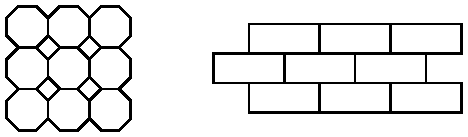
\includegraphics{../graphics/semiRegTess.pdf}
\]
On the left we have a tessellation of a square and an octagon. On the
right we have a ``brick-like'' tessellation.

\begin{dfn}\index{tessellation!regular}\index{regular!tessellation}
A tessellation is called a \textbf{regular tessellation} if it is
composed of copies of a single regular polygon and these polygons meet
vertex to vertex.\index{regular!polygon}
\end{dfn}


\begin{eg} Here are some examples of regular tessellations:
\[
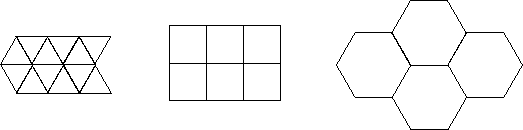
\includegraphics{../graphics/regtess.pdf}
\]
\end{eg}

Johannes Kepler\index{Kepler, Johannes}, who lived from 1571--1630,
was one of the first people to study tessellations. He certainly knew
the next theorem:

\begin{thm} There are only $3$ regular tessellations.
\end{thm}

\begin{ques} Why is the theorem above true?
\end{ques}
\QM

Since one can prove that there are only three regular tessellations,
and we have shown three above, then that is all of them. On the other
hand there are lots of nonregular tessellations. Here are two
different ways to tessellate the plane with a
triangle:\index{tessellation!triangles}
\[
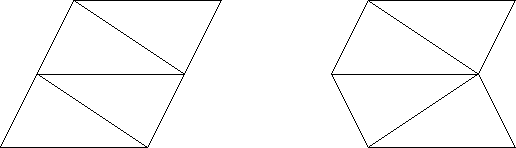
\includegraphics{../graphics/triangletess.pdf}
\]
Here is a way that you can tessellate the plane with any old
quadrilateral:
\[\index{tessellation!any quadrilateral}\index{quadrilateral!tessellation of}
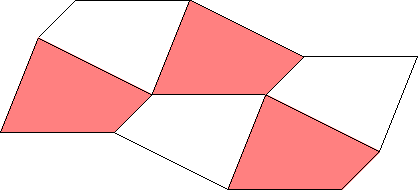
\includegraphics{../graphics/quadtess.pdf}
\]

\subsection{Tessellations and Art}

How does one make art with tessellations? To start, a little
decoration goes a long way. Check this out: Decorate two squares as
such:
\[
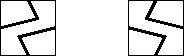
\includegraphics{../graphics/lightningsquares.pdf}
\]
Tessellate them randomly in the plane to get this lightning-like picture:
\[
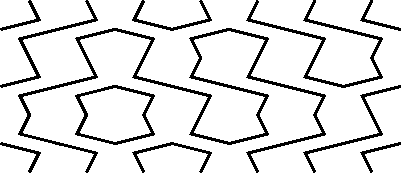
\includegraphics{../graphics/lightningtess.pdf}
\]
\begin{ques} 
What sort of picture do you get if you tessellate these decorated
squares randomly in a plane?
\[
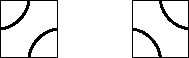
\includegraphics{../graphics/watersquares.pdf}
\]
\end{ques}
\QM

Another way to go is to start with your favorite tessellation:
\[
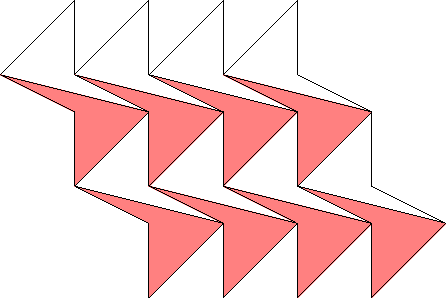
\includegraphics{../graphics/nonconvextess.pdf}
\]
Then you modify it a bunch to get something different:
\[
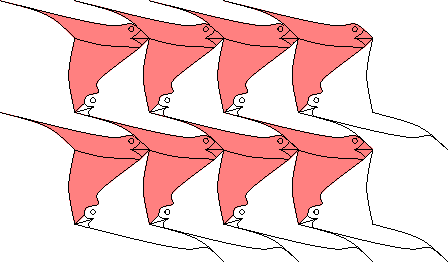
\includegraphics{../graphics/birdstess.pdf}
\]

\begin{ques} What kind of art can you make with tessellations?
\end{ques}
\QM


I'm not a very good artist, but I am a mathematician. So let's use a
tessellation to give a proof! Let me ask you something:

\begin{ques} What is the most famous theorem in mathematics? 
\end{ques}
Probably the Pythagorean Theorem comes to mind. Let's recall the statement of the Pythagorean Theorem:

\begin{thm}[Pythagorean Theorem]\index{Pythagorean Theorem} Given a right triangle, the sum of the squares of the 
lengths of the two legs equals the square of the length of 
the hypotenuse.  Symbolically, if $a$ and $b$ represent the 
lengths of the legs and $c$ is the length of the hypotenuse, 
\[
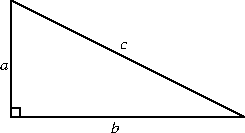
\includegraphics{../graphics/pbppyth.pdf}
\]
then 
\[
a^2 + b^2 = c^2.
\]
\end{thm}


Let's give a proof! Check out this tessellation involving $2$ squares:
\[
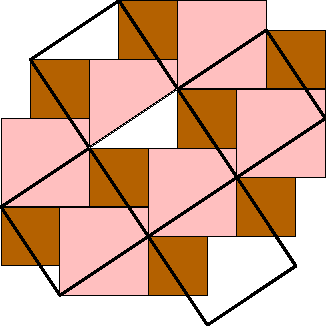
\includegraphics{../graphics/pbppyth2.pdf}
\]
\begin{ques} How does the picture above ``prove'' the Pythagorean Theorem?
\end{ques}
\begin{proof}[Solution]  
The white triangle is our right triangle. The area of the middle
overlaid square is $c^2$, the area of the small dark squares is $a^2$,
and the area of the medium lighter square is $b^2$. Now label all the
``parts'' of the large overlaid square:
\[
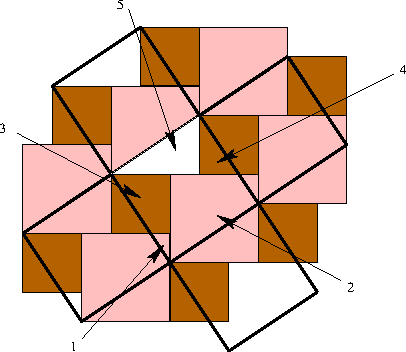
\includegraphics{../graphics/pbppyth2a.pdf}
\]
From the picture we see that
\begin{align*}
a^2 &= \{\text{3 and 4}\}\\
b^2 &= \{\text{1, 2, and 5}\}\\
c^2 &= \{\text{1, 2, 3, 4, and 5}\}
\end{align*}
Hence
\[
c^2 = a^2 + b^2
\]
Since we can always put two squares together in this pattern, this
proof will work for any right triangle.
\end{proof}

\begin{ques} Can you use the above tessellation to give a dissection proof of the Pythagorean Theorem?
\end{ques}
\QM








\newpage

\problems
\begin{enumerate}
\item Show two different ways of tessellating the plane with a given scalene triangle. Label your picture as necessary.
\item Show how to tessellate the plane with a given quadrilateral. Label your picture.
\item Show how to tessellate the plane with a nonregular hexagon. Label your picture.
\item Give an example of a polygon with $9$ sides that tessellates the plane.
\item Give examples of polygons that tessellate and polygons that do
  not tessellate.
\item Give an example of a triangle that tessellates the plane where
  both $4$ and $8$ angles fit around each vertex.
\item True or False: Explain your conclusions.
\begin{enumerate}
\item There are exactly 5 regular tessellations.
\item Any quadrilateral tessellates the plane.
\item Any triangle will tessellate the plane.
\item If a triangle is used to tessellate the plane, then it is always
  the case that exactly $6$ angles will fit around each vertex.
\item If a polygon has more than 6 sides, then it cannot tessellate the plane.
\end{enumerate}
\item Given a regular tessellation, what is the sum of the angles
  around a given vertex?
\item Given that the regular octagon has $135$ degree angles, explain
  why you cannot give a regular tessellation of the plane with a
  regular octagon.
\item \label{tesstable} Fill in the following table:
\begin{center}
\begin{tabular}{|c || c| c| c|}\hline
 Regular & Does it      &  Measure & If it tessellates, how  \\
 $n$-gon & tessellate?  &  of an angle &  many surround each vertex?  \\
\hline\hline
$3$-gon &  &  &  \\ \hline
$4$-gon &  &  &  \\ \hline
$5$-gon &  &  &  \\ \hline
$6$-gon &  &  &  \\ \hline
$7$-gon &  &  &  \\ \hline
$8$-gon &  &  &  \\ \hline
$9$-gon &  &  &  \\ \hline
$10$-gon &  &  &  \\ \hline
\end{tabular}
\end{center}
Hint: A regular $n$-gon has interior angles of $180(n-2)/n$ degrees. 
\begin{enumerate}
\item What do the shapes that tessellate have in common?
\item Make a graph with the number of sides of an $n$-gon on the
  horizontal axis and the measure of a single angle on the vertical
  axis. Briefly describe the relationship between the number of sides
  of a regular $n$-gon and the measure of one of its angles.
\item What regular polygons \textit{could} a bee use for building
  hives? Give some reasons that bees seem to use hexagons.\index{bees}
\end{enumerate}
\item Considering that the regular $n$-gon has interior angles of
  $180(n-2)/n$ degrees, and Problem \ref{tesstable} above, prove that
  there are only 3 regular tessellations of the plane.
\item Explain how the following picture ``proves'' the Pythagorean
  Theorem.
\[
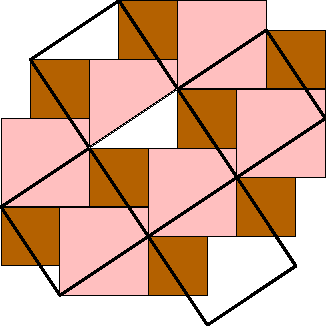
\includegraphics{../graphics/pbppyth2.pdf}
\]
\end{enumerate}









\newpage



\symbolfootnote[0]{Most of the \textit{pictures} from this section are adapted from the wonderful source books: \cite{nelsen} and \cite{nelsen1}.}
\section{Proof by Picture}


Pictures generally do not constitute a proof on their own. However, a
good picture can show insight and communicate concepts better than
words alone. In this section we will show you pictures giving the idea
of a proof and then ask you to supply the words to finish off the
argument. 


\subsection{Proofs Involving Right Triangles}

Let's start with something easy:

\begin{ques} Explain how the following picture ``proves'' that
  the area of a right triangle is half the base times the height.
\[
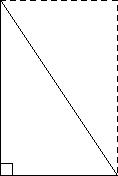
\includegraphics{../graphics/pbpAreaRight.pdf}
\]
\end{ques}
\QM 

That wasn't so bad was it? Now for a game of \textit{whose-who}:

\begin{ques} What is the most famous theorem in mathematics? 
\end{ques}
Probably the Pythagorean Theorem comes to mind. Let's recall the statement of the Pythagorean Theorem:

\begin{thm}[Pythagorean Theorem]\index{Pythagorean Theorem} Given a right triangle, the sum of the squares of the 
lengths of the two legs equals the square of the length of 
the hypotenuse.  Symbolically, if $a$ and $b$ represent the 
lengths of the legs and $c$ is the length of the hypotenuse, 
\[
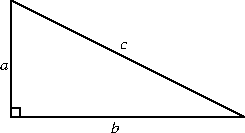
\includegraphics{../graphics/pbppyth.pdf}
\]
then 
\[
a^2 + b^2 = c^2.
\]
\end{thm}
\begin{ques} What is the converse to the Pythagorean Theorem? Is it true? How do you prove it?
\end{ques}
\QM

While everyone may know the Pythagorean Theorem, not as many know how to prove it. Euclid's proof goes kind of like this: 

Consider the following picture:
\[
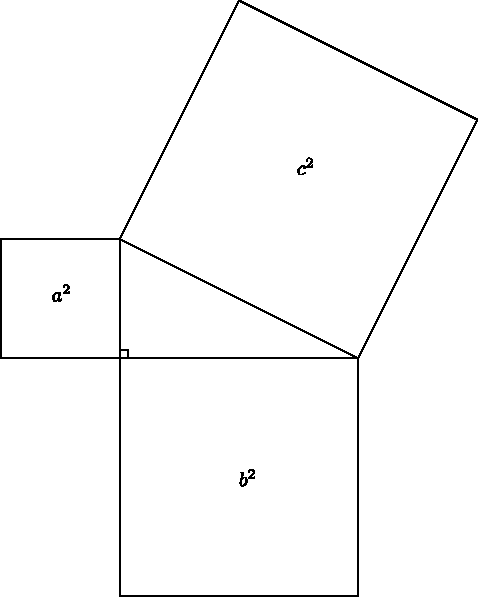
\includegraphics{../graphics/pbppythsqr.pdf}
\]
Now, cut up the squares $a^2$ and $b^2$ in such a way that they fit into $c^2$ perfectly. When you give a proof that involves cutting up the shapes and putting them back together, it is called a \textbf{dissection proof}.\index{dissection proof} The trick to ensure that this is actually a proof is in making sure
that your dissection will work no matter what right triangle you are
given. Does it sound complicated? Well it can be. 


Is there an easier proof?  Sure, look at:
\[
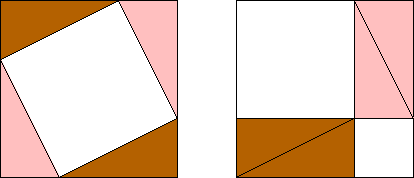
\includegraphics{../graphics/pbppyth1.pdf}
\]
\begin{ques} How does the picture above ``prove'' the Pythagorean Theorem?
\end{ques}


\begin{proof}[Solution] Both of the large squares above are the same size. Moreover both the unshaded regions above must have the same area. The large white square on the left has an area of $c^2$ and the two white squares on the right have a combined area of $a^2 + b^2$. Thus we see that:
\[
c^2 = a^2 + b^2
\]
\end{proof}


Now a paradox:

\begin{para}\index{paradox!triangle dissection} What is wrong with this picture?
\[
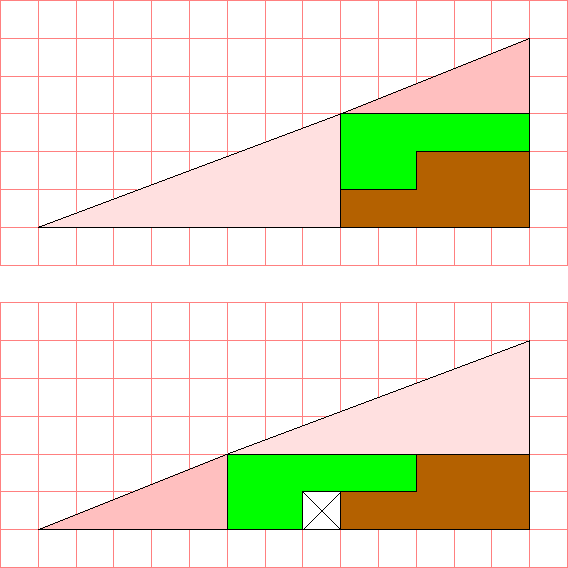
\includegraphics{../graphics/triparadox.pdf}
\]
\end{para}

\begin{ques} How does this happen\footnote{See \cite{gardner2} Chapter 8, for a wonderful discussion of puzzling pictures like this one.}?
\end{ques}
\QM

\subsection{Proofs Involving Boxy Things}

Consider the problem of \textit{Doubling the Cube}.\index{doubling the cube} If a mathematician asks us to double a cube, he or she is asking us to double the \textbf{volume} of a given cube. One may be tempted to merely double each side, but this doesn't double the volume! 

\begin{ques} Why doesn't doubling each side of the cube double the volume of the cube? 
\end{ques}
\QM

Well, let's answer an easier question first. How do you double the area of a square? Does taking each side and doubling it work? 
\[
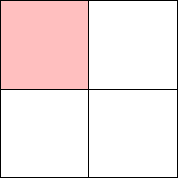
\includegraphics{../graphics/pbpsquare.pdf}
\]
No!  You now have four times the area. So you \textbf{cannot} double the area of a square merely by doubling each side.
What about for the cube? Can you double the volume of a cube merely by doubling the length of every side? Check this out:
\[
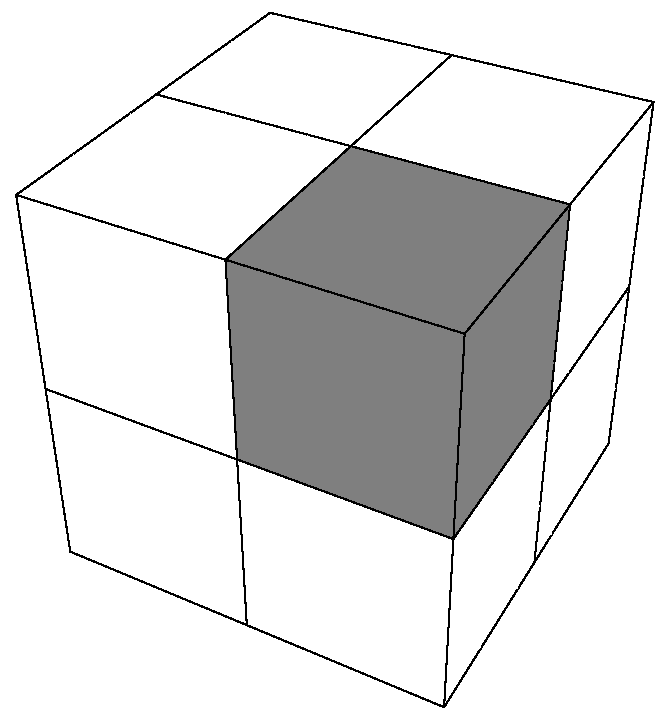
\includegraphics[scale=.4]{../graphics/119VolumeCube.pdf}
\]
Ah, so the answer is again no. If you double each side of a cube you have $8$ times the volume.

\begin{ques}
What happens to the area of a square if you multiply the sides by an
arbitrary integer? What about the volume of a cube? Can you explain
what is happening here?
\end{ques} 
\QM



\subsection{Proofs Involving Infinite Sums}

As is our style, we will start off with a question:

\begin{ques} Can you add up an infinite number of terms and still get a 
finite number?
\end{ques}


Consider $1/3$.  Actually, consider the decimal notation for $1/3$:
\[
\frac{1}{3} = .333333333333333333333333333333\dots
\]
But this is merely the sum:
\[
.3 + .03 + .003 + .0003 + .00003 + .000003 + \cdots
\]
It stays less than $1$ because the terms get so small so 
quickly.  Are there other infinite sums of this sort?  You 
bet! Check out this picture:
\[
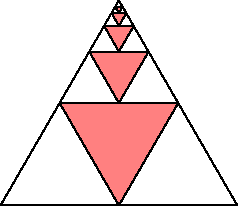
\includegraphics{../graphics/pbptriangle.pdf}
\]
\begin{ques} Explain how the picture above ``proves'' that:
\[
\frac{1}{4} + \left(\frac{1}{4}\right)^2 +  \left(\frac{1}{4}\right)^3 +  \left(\frac{1}{4}\right)^4 +  \left(\frac{1}{4}\right)^5 + \cdots = \frac{1}{3}
\]
\end{ques}

\begin{proof}[Solution] Let's take it in steps.  If the big triangle has area 
$1$, the area of the shaded region below is $1/4$. 
\[
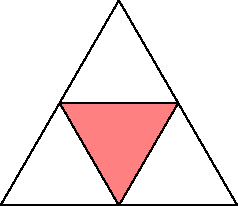
\includegraphics{../graphics/pbptriangle1.pdf}
\]
We also see that the area of the shaded region below 
\[
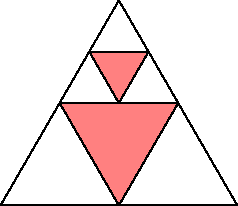
\includegraphics{../graphics/pbptriangle2.pdf}
\]
is:
\[
\frac{1}{4} + \left(\frac{1}{4}\right)^2
\]
Continuing on in this fashion we see that the area of all the shaded regions is:
\[
\frac{1}{4} + \left(\frac{1}{4}\right)^2 +  \left(\frac{1}{4}\right)^3 +  \left(\frac{1}{4}\right)^4 +  \left(\frac{1}{4}\right)^5 + \cdots
\]
But look, the unshaded triangles have twice as much area as 
the shaded triangle.  Thus the shaded triangles must have an
area of $1/3$.
\end{proof}



\subsection{Thinking Outside the Box}


A \textit{calisson}\index{calisson} is a French candy that sort of looks like two equilateral triangles stuck together. They usually come in a hexagon-shaped box. 

\begin{ques} How do the calissons fit into their hexagon-shaped box?
\end{ques}

If you start to put the calissons into a box, you quickly see that they can be placed in there with exactly three different orientations:
\[
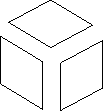
\includegraphics{../graphics/pbporicas.pdf}
\]
\begin{thm}\label{T:cal} In any packing, the number of calissons with a given orientation is exactly one-third the total number of calissons in the box.
\end{thm}

Look at this picture:
\[
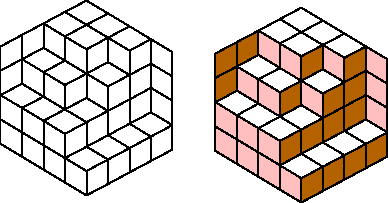
\includegraphics{../graphics/pbpcas.pdf}
\]

\begin{ques} How does the picture above ``prove'' Theorem~\ref{T:cal}? Hint: Think outside the box!
\end{ques}
\QM





\newpage

\subsection*{Problems for Section~\thesection}\hrule\vspace{1ex}
\begin{enumerate}
\item Explain the rule
\[
\text{even} + \text{even} = \text{even}
\]
in two different ways. First give an explanation based on
pictures. Second give an explanation based on algebra. 
\item Explain the rule
\[
\text{odd} + \text{even} = \text{odd}
\]
in two different ways. First give an explanation based on
pictures. Second give an explanation based on algebra.
\item Explain the rule
\[
\text{odd} + \text{odd} = \text{even}
\]
in two different ways. First give an explanation based on
pictures. Second give an explanation based on algebra.
\item Explain the rule
\[
\text{even} \cdot \text{even} = \text{even}
\]
in two different ways. First give an explanation based on
pictures. Second give an explanation based on algebra.
\item Explain the rule
\[
\text{odd} \cdot \text{odd} = \text{odd}
\]
in two different ways. First give an explanation based on
pictures. Second give an explanation based on algebra.
\item Explain the rule
\[
\text{odd} \cdot \text{even} = \text{even}
\]
in two different ways. First give an explanation based on
pictures. Second give an explanation based on algebra.
\item\label{P:RTA} Explain how the following picture ``proves'' that
  the area of a right triangle is half the base times the height.
\[
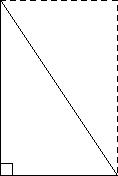
\includegraphics{../graphics/pbpAreaRight.pdf}
\]

\item Suppose you know that the area of a \textbf{right} triangle is
  half the base times the height. Explain how the following picture
  ``proves'' that the area of \textbf{every} triangle is half the base times the
  height.
\[
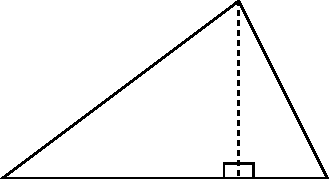
\includegraphics{../graphics/pbpDisTri.pdf}
\]
Now suppose that a student, say \textit{Geometry Giorgio} attempts to
solve a similar problem. Again knowing that the area of a right
triangle is half the base times the height, he draws the following
picture:
\[
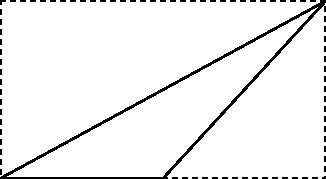
\includegraphics{../graphics/pbpDisTriGio.pdf}
\]
\textit{Geometry Giorgio} states that the diagonal line cuts the
rectangle in half, and thus the area of the triangle is half the base
times the height. Is this correct reasoning? If so, give a complete
explanation. If not, give correct reasoning based on \textit{Geometry
  Giorgio}'s picture.


\item Suppose you know that the area of a \textbf{right} triangle is
  half the base times the height. Explain how the following picture
  ``proves'' that the area of any triangle is half the base times the
  height. Note, this way of thinking is the basis for Cavalieri's
  Principle.\index{Cavalieri's Principle}
\[
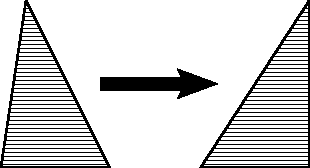
\includegraphics{../graphics/pbpShearTri.pdf}
\]
\item Explain how the following picture ``proves'' that the area of
  any parallelogram is base times height. Note, this way of thinking
  is the basis for Cavalieri's Principle.\index{Cavalieri's Principle}
\[
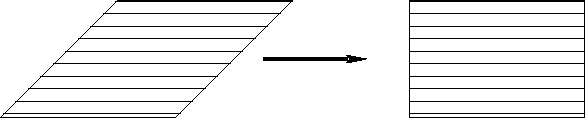
\includegraphics{../graphics/pbpShearPara.pdf}
\]

\item Explain how to use a picture to ``prove'' that a triangle of a
  given area could have an arbitrarily large perimeter.

\item Give two explanations of how the following picture ``proves''
  the Pythagorean Theorem, one using algebra and one without algebra. 
\[
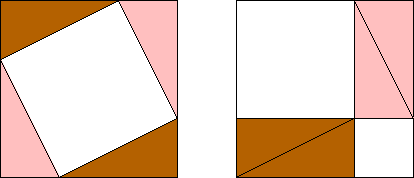
\includegraphics{../graphics/pbppyth1.pdf}
\]
\item Give two explanations of how the following picture ``proves''
  the Pythagorean Theorem, one using algebra and one without algebra. 
\[
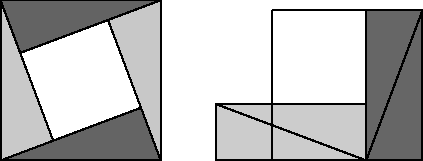
\includegraphics{../graphics/pbppyth3.pdf}
\]
\item Explain how the following picture ``proves'' the Pythagorean Theorem.
\[
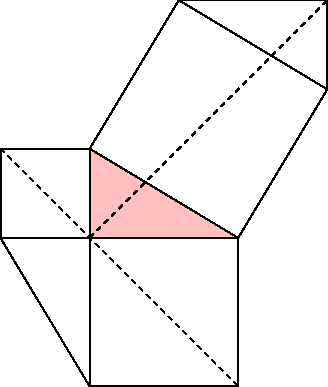
\includegraphics{../graphics/pbpdavinci.pdf}
\]
Note: This proof is due to Leonardo da Vinci.
%\item Explain how the following picture ``proves'' the Pythagorean Theorem.
%\[
%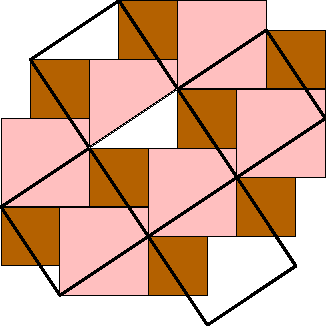
\includegraphics{../graphics/pbppyth2.pdf}
%\]
%\item Use the following tessellation to give a dissection proof of the Pythagorean Theorem.
%\[
%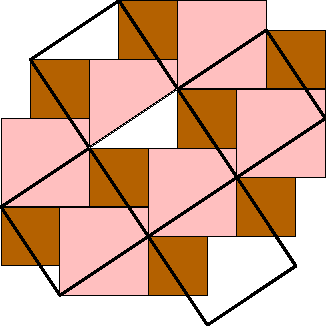
\includegraphics{../graphics/pbppyth2.pdf}
%\]
%\item Explain how the following picture ``proves'' the Pythagorean Theorem.
%\[
%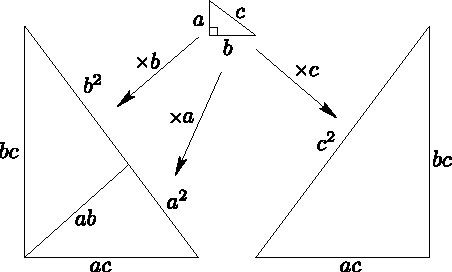
\includegraphics{../graphics/pbpdilation.pdf}
%\]
\item\label{P:pbptrap} Recall that a trapezoid is a quadrilateral with two parallel sides. Consider the following picture:
\[
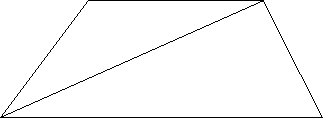
\includegraphics{../graphics/trap.pdf}
\]
How does the above picture prove that the area of a trapezoid is
\[
\mathrm{area}= \frac{h(b_1 + b_2)}{2},
\]
where $h$ is the height of the trapezoid and $b_1$, $b_2$, are the lengths of the parallel sides?
\item Explain how the following picture ``proves'' the Pythagorean Theorem.
\[
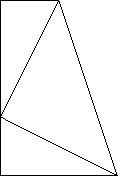
\includegraphics{../graphics/pbptrap.pdf}
\]
Note: This proof is due to James A.\ Garfield, the 20th President of the United States.
\item Look at Problem~\ref{P:pbptrap}. Can you use a similar picture
  to prove that the area of a parallelogram
\[
\includegraphics{../graphics/para.pdf}
\]
is the length of the base times the height?
\item Explain how the following picture ``proves'' that the area of a
  parallelogram is base times height.
\[
\includegraphics{../graphics/para3.pdf}
\]
Now suppose that a student, say \textit{Geometry Giorgio} attempts to
solve a similar problem. In an attempt to prove the formula for the
area of a parallelogram, \textit{Geometry Giorgio} draws the following
picture:
\[
\includegraphics{../graphics/paragiorgio.pdf}
\]
At this point \textit{Geometry Giorgio} says that he has proved the
formula for area of a parallelogram. What do you think of his picture?
Give a complete argument based on his picture.

\item Which of the above ``proofs'' for the formula for the area of a
  parallelogram is your favorite? Explain why.

\item Explain how the following picture ``proves'' that the area of a
  quadrilateral is equal to half of the area of the parallelogram
  whose sides are parallel to and equal in length to the diagonals of
  the original quadrilateral.
\[
\includegraphics[scale=.7]{../graphics/pbpquadarea.pdf}
\]

\item Explain how the following picture ``proves'' that if a
  quadrilateral has two opposite angles that are equal, then the
  bisectors of the other two angles are parallel or on top of each
  other.
\[
\includegraphics[scale=.7]{../graphics/119hw5_2.pdf}
\]



\break

\item\label{P:Tparadox1} Why might someone find the following picture
  disturbing? How would you assure them that actually everything is
  good and well in the geometrical world?
\[
\includegraphics[scale=.8]{../graphics/triparadox.pdf}
\]



\item\label{P:Tparadox2} Why might someone find the following picture
  disturbing? How would you assure them that actually everything is
  good and well in the geometrical world?
\[
\includegraphics[scale=.8]{../graphics/triparadox2.pdf}
\]


\item How could you explain to someone that doubling the lengths of each side of a cube does not double the volume of the cube?

\item\label{P:sq1}  Explain how the following picture ``proves'' that:
\[
\frac{1}{2} + \left(\frac{1}{2}\right)^2 +  \left(\frac{1}{2}\right)^3 +  \left(\frac{1}{2}\right)^4 +  \left(\frac{1}{2}\right)^5 + \cdots = 1
\]
\[
\includegraphics{../graphics/pbpsqgeo.pdf}
\]
\item\label{P:sq2}  Explain how the following picture ``proves'' that if $0 < r < 1$:
\[
r + r(1-r) + r(1-r)^2 + r(1-r)^3 + \cdots = 1
\]
\[
\includegraphics{../graphics/pbpgengeo.pdf}
\]
\item\label{P:tri1} Explain how the following picture ``proves'' that:
\[
\frac{1}{4} + \left(\frac{1}{4}\right)^2 +  \left(\frac{1}{4}\right)^3 +  \left(\frac{1}{4}\right)^4 +  \left(\frac{1}{4}\right)^5 + \cdots = \frac{1}{3}
\]
\[
\includegraphics{../graphics/pbptriangle.pdf}
\]
\item Considering Problem~\ref{P:sq1}, Problem~\ref{P:sq2}, and
  Problem~\ref{P:tri1} can you give a new picture ``proving'' that: 
\[
\frac{1}{4} + \left(\frac{1}{4}\right)^2 +  \left(\frac{1}{4}\right)^3 +  \left(\frac{1}{4}\right)^4 +  \left(\frac{1}{4}\right)^5 + \cdots = \frac{1}{3}
\]
Carefully explain the connection between your picture and the
mathematical expression above.

\item Explain how the following picture ``proves'' that  in any packing, the number of calissons with a given orientation is exactly one-third the total number of calissons in the box.
\[
\includegraphics{../graphics/pbpcas.pdf}
\]
\end{enumerate}
